\documentclass{article}

% if you need to pass options to natbib, use, e.g.:
%     \PassOptionsToPackage{numbers, compress}{natbib}
% before loading neurips_2019

% ready for submission
% \usepackage{neurips_2019}

% to compile a preprint version, e.g., for submission to arXiv, add add the
% [preprint] option:
    % \usepackage[preprint]{neurips_2019}

% to compile a camera-ready version, add the [final] option, e.g.:
     \usepackage[nonatbib, final]{neurips_2020}

% to avoid loading the natbib package, add option nonatbib:
%     \usepackage[nonatbib]{neurips_2019}

\usepackage[utf8]{inputenc} % allow utf-8 input
\usepackage[T1]{fontenc}    % use 8-bit T1 fonts
\usepackage{hyperref}       % hyperlinks
\usepackage{url}            % simple URL typesetting
\usepackage{booktabs}       % professional-quality tables
\usepackage{nicefrac}       % compact symbols for 1/2, etc.
\usepackage{microtype}      % microtypography
\usepackage{graphicx}
\usepackage{caption}
\usepackage{subcaption}
\usepackage{float}
\usepackage[ruled,vlined]{algorithm2e}
\usepackage{inputenc, amsmath, amsfonts, amssymb, biblatex}
\addbibresource{references.bib}

\title{An Application of Convolutional Neural Networks for COVID-19 CT Scan Classification}
\author{
  Cullen Pu \\
  University of Toronto \\
  \texttt{cullen.pu@mail.utoronto.ca} \\
  \And
  Alexander Shih \\
  University of Toronto \\
  \texttt{alexander.shih@mail.utoronto.ca} \\
  \And
  Sijia Cai \\
  University of Toronto \\
  \texttt{s.cai@mail.utoronto.ca} \\
}
\date{April 20, 2021}

\begin{document}

\maketitle

\begin{abstract}
    The demand for efficient COVID-19 detection methods is evident as the pandemic continues to devastate our communities. In this paper, we compare the performance of several convolutional models, including ResNet \cite{ResNet}, DenseNet \cite{DenseNet}, and InceptionNet \cite{Inception}, with transfer learning to classify between COVID-19 cases and normal cases using a limited dataset of chest CT scans. Our results show that DenseNet-121 works the best for this classification problem, achieving over 94\% test accuracy.
\end{abstract}

\section{Introduction}
With the advent of the COVID-19 pandemic, the need for fast and reliable diagnostic tools to detect afflicted individuals becomes increasingly urgent not only to maintain the health of the general public, but also to provide early assistance to higher risk individuals. Since COVID-19 is a disease that affects the respiratory system, we propose using chest scans as a possible alternative method to diagnose COVID-19, thereby minimizing healthcare practitioners' direct contact with symptomatic patients and their bodily fluids compared to current methods such as PCR testing.

We propose repurposing, fine-tuning, and comparing the performances of COVID-19 detection on chest CT scans from a variety of existing Convolutional Neural Networks. Specifically, we will use the ResNet-18, ResNet-50 \cite{ResNet}, DenseNet-121, DenseNet-161 \cite{DenseNet}, and Inception \cite{Inception} models and apply transfer learning. The scans will be sourced from a dataset of 2482 images with 1230 normal chest scans and 1252 COVID-19 chest scans compiled by Eduardo Soares and Plamen Angelov of Lancaster University. It was collected from patients from hospitals in Sao Paulo, Brazil, and made publicly available for research. \cite{PlamenEduardo}.

\section{Related Works}
Previous research has been conducted in the area of detecting pneumonia from digitial x-ray images. Rahman et. al achieved extremely promising results using four pre-trained CNNs, AlexNet \cite{AlexNet}, ResNet \cite{ResNet}, DenseNet \cite{DenseNet}, and SqueezeNet \cite{SqueezeNet} in classifying between normal, bacterial pneumonial, and viral pneumonial chest x-ray images, reaching a classification accuracy of 98\%, 95\%, and 93.3\%, respectively \cite{Rahman_2020}.

In November of 2020, Wang et. al introduced COVID-Net, one of the first open source CNN architectures specifically designed to detect COVID-19 cases from COVIDx, an aggregation of open source chest x-ray images \cite{Wang2020}. COVID-Net was able to achieve 93.3\% test accuracy, highlighting the effectiveness of using deep learning to rapidly generate a solution in response to urgent situations.

As mentioned before, the original publishers of the dataset also proposed a deep learning model using an eXplainable Deep Learning approach (xDNN) \cite{xie2020explainable}. They achieved an F1 score of 97.31\% \cite{Soares2020}. We use their model as on the limited-size dataset as a benchmark to measure the efficacy of our best performing repurposed models.

\section{Method}
We use CNN models because they are currently the state of the art models for image recognition. AlexNet is considered an outdated model, which is why we chose not to use AlexNet for these tests. ResNet in particular is a powerful deep residual network capable of having many more layers than a traditional CNN, made possible by its use of residual blocks which solve the vanishing gradient problem. There are different ResNet sizes, ranging from the smallest, ResNet-18, being 18 layers deep, up to the 152 layer ResNet-152 \cite{ResNet}. Because ResNet was originally trained to classify between 1000 classes and our COVID-19 classification problem involves binary classification, we decide to use ResNet-18, the smallest variant. In contrast, we also use ResNet-50, a popular middle-ground variant of ResNet, to see if a greater depth achieves better performance in this binary classification problem.

DenseNet was proposed after ResNet and can be thought of as an extension of ResNet. DenseNet uses multi-layer feature concatenation, in which each layer obtains inputs from all previous layers and also connects to all later layers. It requires fewer parameters, provides better accuracy, and allows for more depth than a traditional CNN \cite{DenseNet}. Like with ResNet, we train on two different DenseNet sizes, DenseNet-121 and DenseNet-161, and compare which performs better.

InceptionNet is another widely used image recognition model which pushed breakthroughs in image recognition and detection. With a focus on reducing the computational cost in CNNs, it utilizes factorized convolutions and aggressive regularization \cite{Inception}. It uses less layers and is therefore less prone to overfitting. We will also be using Inception v3 for our COVID-19 classification problem.


\begin{algorithm}[H]
\caption{The following algorithm shows our training loop and how we calculate false positives and negatives.}
\SetAlgoLined
    \ForEach{epoch}{
    \ForEach{phase in [``train", ``validate"]}{
        total\_loss = total\_correct = 0\;
        false\_positives = false\_negatives = total\_covid = total\_healthy = 0\;

        \ForEach{batch in dataloader.phase}{
            Run forward pass and get model predictions\;
            \textbf{Calculate} Cross Entropy Loss\;
            Backpropagate\;
            \textbf{Update} total\_loss, total\_correct\;
            \textbf{Update} false\_positives, false\_negatives, total\_healthy, total\_covid\;
            
        }
        epoch\_loss = total\_loss / len(dataloader.phase)\;
        accuracy = total\_correct / len(dataloader.phase)\;
        false\_positive\_rate = false\_positives / (false\_positives + total\_healthy)\;
        false\_negative\_rate = false\_negative / (false\_negative + total\_covid)\;
    }
    }
\end{algorithm}

% \begin{verbatim}
    
% \end{verbatim}

\section{Experiments}
We fine tuned ResNet-18 by adding sequential linear layers. For ResNet-18, we replaced the original fully connected layer with three fully connected layers of size 512, 128, and 32 respectively. Since it was the shallowest of the models we tested it is the least prone to overfitting so we added more fully connected layers. When repurposing ResNet-50, we added only two fully connected layers: one of size 2048 and one of size 1024 since it is a larger model than ResNet-18.

We repurposed both DenseNet-121 and DenseNet-161 by replacing the last layer with only a single fully connected layer with two outputs. Loss plots were closely monitored and early stopping was used to prevent overfitting the test dataset. We found that a lower learning rate worked better on DenseNet-161 because it lead to much less fluctuation in the validation loss, usually a telltale sign of overfitting.

Inception v3 was repurposed in the same way as DenseNet, with only a single fully connected layer with two outputs replacing the last layer. We do so because one of the main benefits of Inception v3 is it's efficiency; to preserve this, we add just one fully connected layer to avoid adding many new connections to the model.

All 5 models were trained using the Adam optimizer with weight decay \cite{kingma2017adam}.

\section{Results}
Out of all the models, the one that was able to best classify between COVID-19 and non COVID-19 cases was DenseNet-121, which achieved a test accuracy of 94.38\%. Nonetheless, in practicality and especially in the medical field, classification accuracy is not the sole important factor. As a method to quickly determine if a patient may have COVID-19 and require further testing and treatment, this type of model must also achieve a low False Negative Rate (FNR).
\begin{table}[h]
\centering
\caption{Model Performance}
\begin{tabular}{lcccccc}
\toprule
    Model & Val Accuracy & Test Loss & Test Accuracy & False Positive & False Negative \\
    \midrule
    ResNet-18 & 0.8911 & 0.2358 & 0.8835 & 0.1189 & 0.0889 \\
    \addlinespace
    ResNet-50 & 0.8710 & 0.2132 & 0.9116 & 0.1490 & 0.0077 \\
    \addlinespace
    DenseNet-121 & 0.8891 & 0.1944 & 0.9438 & 0.0725 & 0.032 \\
    \addlinespace
    DenseNet-161 & 0.8810 & 0.3077 & 0.8916 & 0.1194 & 0.0775 \\
    \addlinespace
    Inception v3 & 0.8871 & 0.3145 & 0.8635 & 0.1357 & 0.1049 \\
\bottomrule
\end{tabular}
\end{table}

The model that achieved the lowest FNR is ResNet-50, with a test FNR of 0.77\%. Interestingly, ResNet-50 was also the model that achieved the highest False Positive Rate (FPR) of 14.9\%. A high False Positive Rate is also undesirable in the medical field because it could lead to a waste of resources and emotional stress on healthy patients. However, due to fluctuations in its loss and accuracy graph, we do not believe that this would be the most effective model. Rather, DenseNet-121 was the most stable in terms of both accuracy and loss and still performed very well on the test data, with a still low false negative rate of 0.032.

Surprisingly, Inception v3 performed the worst overall; it achieved a final test accuracy of 86.35\%, FPR of 13.57\%, and FNR of 10.49\%. This could be because InceptionNet seeks to reduce computational cost in CNNs. However, with a small dataset like ours, computational cost is not very expensive, so this factor was never accounted for.

Another notable result was the effect of overfitting - or lack thereof. The more parameters a model has, the more prone overfitting is to occur. In addition, since our problem is binary classification, a larger model is even more likely to overfit, harming performance. This was the case for DenseNet, as DenseNet-121 outperformed DenseNet-161, and generally for ResNet, where ResNet-18 overall had lower loss and higher accuracy on the validation set. Our results show the models with fewer parameters performed better overall, as expected.

Comparing between models, it is clear that DenseNet was the best performing model as its accuracy increased over the epochs and did not fluctuate as much as the other models. This is likely because DenseNet utilizes connecting layers in a feed-forward method where the feature maps of previous layers are used as inputs for each layer. A benefit is that it drastically reduces the number of parameters for the model, which is likely why it performed so well compared to the other models, as it likely resulted in less overfitting.

\begin{figure}[H]
    \centering
    \begin{subfigure}[b]{0.30\textwidth}
            \centering
            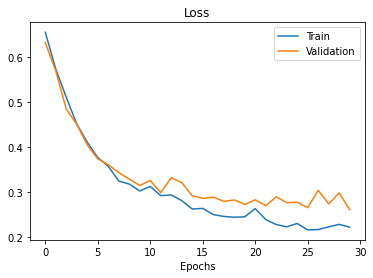
\includegraphics[width=.85\linewidth]{images/resnet18_loss}
            \caption{ResNet-18}
            \label{ResNet-18}
    \end{subfigure}%
    \begin{subfigure}[b]{0.30\textwidth}
            \centering
            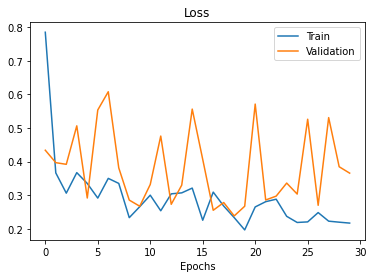
\includegraphics[width=.85\linewidth]{images/resnset50_loss}
            \caption{ResNet-50}
            \label{ResNet-50}
    \end{subfigure}%
    \begin{subfigure}[b]{0.30\textwidth}
            \centering
            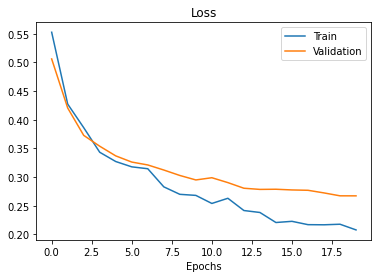
\includegraphics[width=.85\linewidth]{images/densenet121_loss}
            \caption{DenseNet-121}
            \label{DenseNet-121}
    \end{subfigure} \\
    \begin{subfigure}[b]{0.30\textwidth}
            \centering
            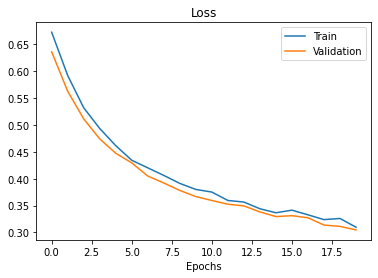
\includegraphics[width=.85\linewidth]{images/densenet161_loss}
            \caption{DenseNet-161}
            \label{DenseNet-161}
    \end{subfigure}%
    \begin{subfigure}[b]{0.30\textwidth}
            \centering
            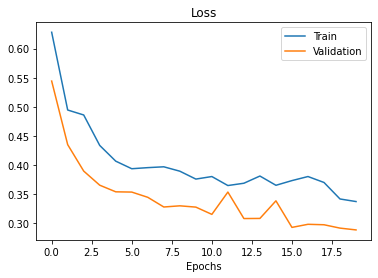
\includegraphics[width=.85\linewidth]{images/inceptionv3_loss.png}
            \caption{Inception v3}
            \label{Inception v3}
    \end{subfigure}
    \caption{Model Loss}\label{fig:animals}
\end{figure}
\begin{figure}[H]
    \centering
    \begin{subfigure}[b]{0.30\textwidth}
            \centering
            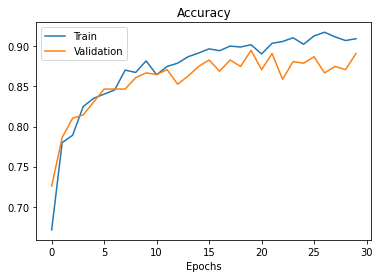
\includegraphics[width=.85\linewidth]{images/resnet18_acc}
            \caption{ResNet-18}
            \label{ResNet-18}
    \end{subfigure}%
    \begin{subfigure}[b]{0.30\textwidth}
            \centering
            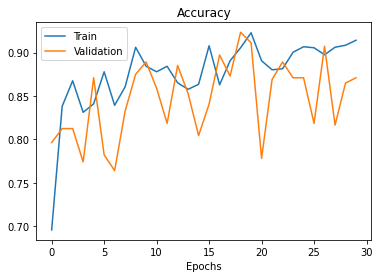
\includegraphics[width=.85\linewidth]{images/resnset50_acc}
            \caption{ResNet-50}
            \label{ResNet-50}
    \end{subfigure}%
    \begin{subfigure}[b]{0.30\textwidth}
            \centering
            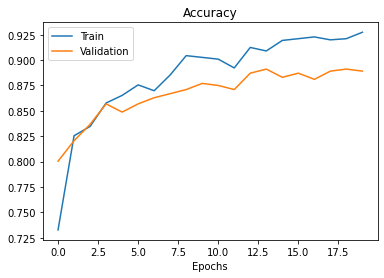
\includegraphics[width=.85\linewidth]{images/densenet121_acc}
            \caption{DenseNet-121}
            \label{DenseNet-121}
    \end{subfigure} \\
    \begin{subfigure}[b]{0.30\textwidth}
            \centering
            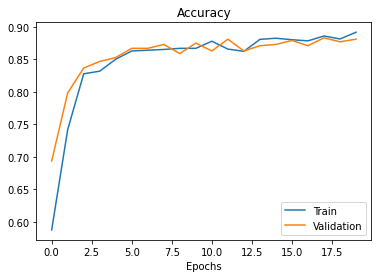
\includegraphics[width=.85\linewidth]{images/densenet161_acc}
            \caption{DenseNet-161}
            \label{DenseNet-161}
    \end{subfigure}%
    \begin{subfigure}[b]{0.30\textwidth}
            \centering
            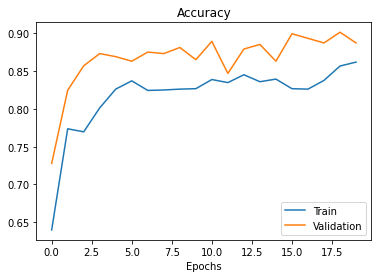
\includegraphics[width=.85\linewidth]{images/inceptionv3_acc.png}
            \caption{Inception v3}
            \label{Inception v3}
    \end{subfigure}
    \caption{Model Accuracy}\label{fig:animals}
\end{figure}

\section{Summary}
The COVID-19 pandemic has caused repercussions around the world that impact our lives. It is evident that we will continue to feel the consequences for years to come. Thus, it is imperative that we continue to develop new methods that can streamline COVID-19 testing in order to mitigate its spread. In this paper, we explored the performance of five pre-trained CNNS, namely ResNet-18, ResNet-50, DenseNet-121, DenseNet-161, and Inception v3, in classifying between COVID-19 and non COVID-19 chest CT scans. From our experiments, we discovered that DenseNet-121 had the highest test accuracy, 94.38\%, with reasonable False Positive and False Negative rates. Other models saw tradeoffs in classification accuracy, FPR, and FNR, which would make them less optimized for medical testing. Additionally, we showed that models that have more parameters tend to overfit on smaller datasets like the one used.

 In conclusion we demonstrate how several existing architectures can achieve satisfactory on new problems using transfer learning. However, for the purposes of medical testing, more specialized technology should be developed. In future work, researchers can also explore how neural networks specifically designed for examining CT scans and other medical imagery perform in classifying COVID-19 chest scans.

\newpage

\section{Attributions}
Cullen Pu wrote the code for the training loop and image visualization. Alex Shih wrote code for loading the dataset and plotting loss. Stella Cai fine tuned many of the models. All three members contributed to the report.

\printbibliography

\end{document}
